\section{Results and Discussion} \label{se:resp1}
         
\subsection{Interaction Energies and Electric Dipole Moments} 
Interaction energies and electric dipole moments computed with the MBE were reported in the previous study\cite{Mach2014} and extensive reviews of the general behavior of the MBE for such properties are available elsewhere (e.g. Ref.~\citenum{Richard2018a} and references therein).  We found that the SSFC correction was insignificant for all cases (see the Supporting Information), except for methyloxirane in a 13-water solvent shell, Fig.\ \ref{metox_13}.
   \begin{figure}
            \begin{subfigure}{.5\textwidth}
                \centering
                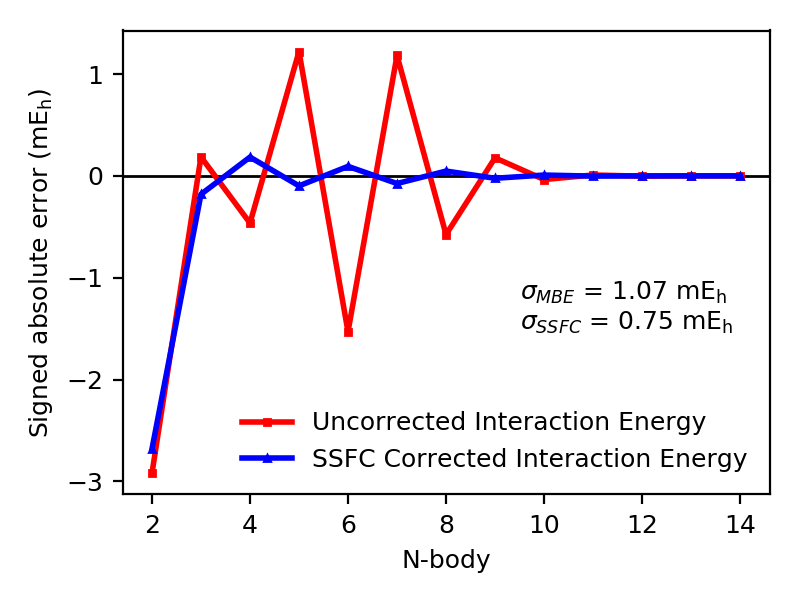
\includegraphics[scale=.75]{p1/graphs/metox_13_int.png}
                \caption{}
                \label{int_e_13}
            \end{subfigure}%
            \begin{subfigure}{.5\textwidth}
                \centering
                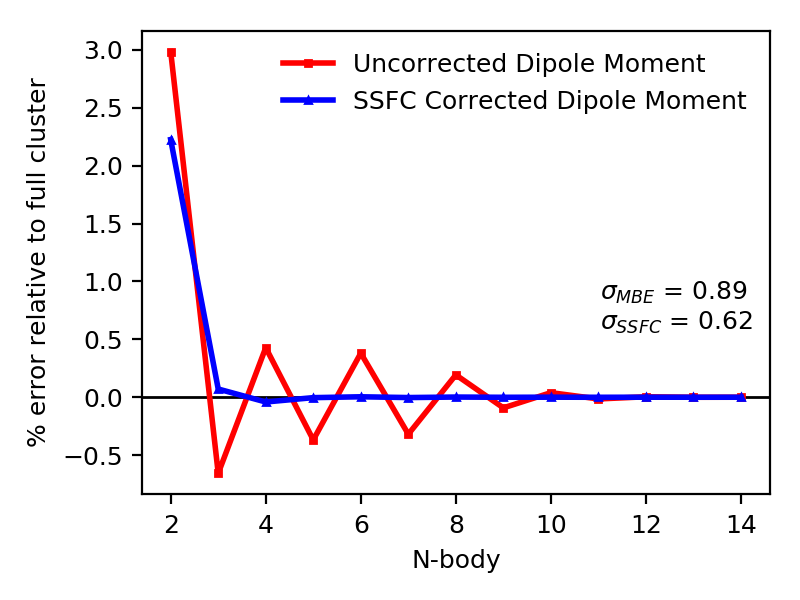
\includegraphics[scale=.75]{p1/graphs/metox_13_dip.png}
                \caption{}
                \label{dip_13}
            \end{subfigure}
            \caption{MBE and SSFC of (a) interaction energies and (b) dipole moments for (\textit{S})-methyloxirane in a 13-water solvent shell.}
            \label{metox_13}
        \end{figure}
        As noted in previous studies of $\sim$ten-body expansions\cite{Ouyang2014,Richard2018a}, oscillating errors in the convergence of the interaction energy in the milli-Hartree range were observed for the methyloxirane system considered. While these oscillations are not as significant as those seen for other properties, the improvement in convergence by the SSFC correction as evidenced by Fig.\ \ref{int_e_13} is still noteworthy. Note that, by definition, the MBE and SSFC interaction energies are different due to the different basis sets used for the monomer terms, so the absolute errors relative to the MBE or SSFC interaction energy are reported. The dipole moment in Fig.\ \ref{dip_13} also exhibits oscillations uncharacteristic of the smaller solvent shells (nearly 0.5\% error even at six-body), and again the SSFC correction dampens the oscillations dramatically. This suggests that the BSSE inherent in the MBE for interaction energies --- and its characteristic increase relative to system size --- is present for other properties as well. If the oscillations observed for higher-order properties in the previous study are indeed indicative of BSSE, then CP corrections should play a major role in damping them.

    \subsection{Dynamic Dipole Polarizabilities}
    Dipole polarizabilities calculated with the MBE were reported for solvated (\textit{S})-methyloxirane, (\textit{M})-dimethylallene, and (\textit{S})-methylthiirane in the previous study\cite{Mach2014} using the B3LYP functional. Their oscillatory behavior has been reproduced here with the CAM-B3LYP functional and CP-corrected with the SSFC method, as shown in Fig.\ \ref{metox_metthi_dma_pol}.
        \begin{figure}
            \begin{subfigure}{0.5\textwidth}
                \centering
                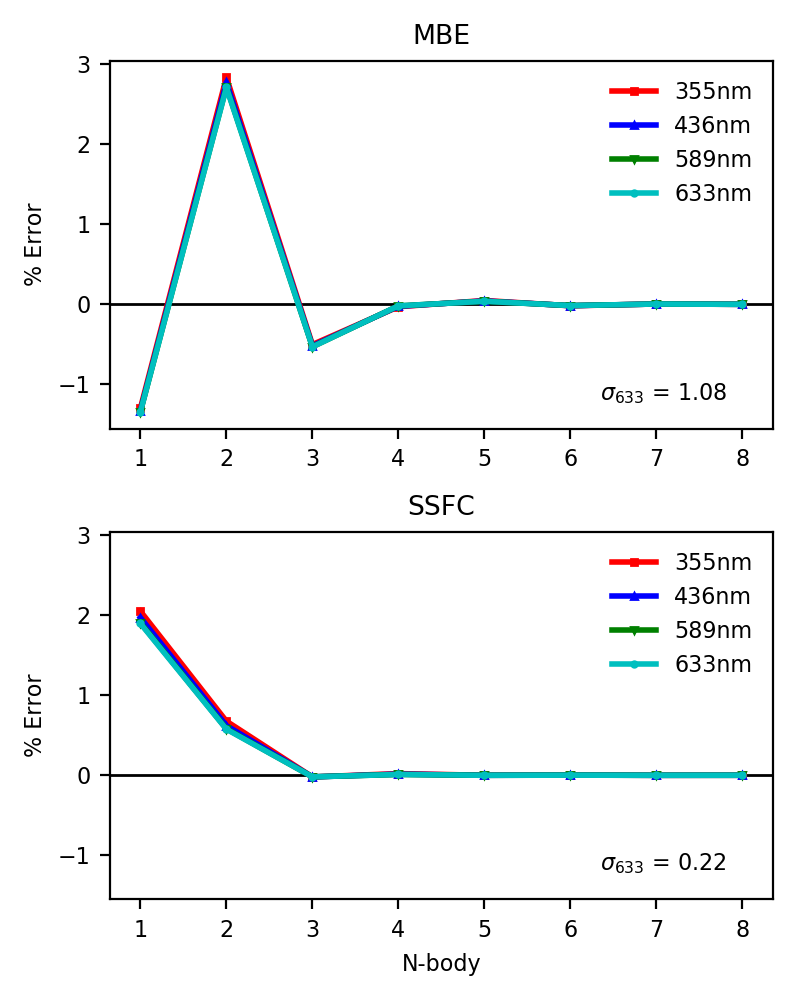
\includegraphics[scale=0.75]{p1/graphs/metox_7_pol.png}
                \caption{(\textit{S})-methyloxirane}
                \label{metox_7_pol}
            \end{subfigure}%
            \begin{subfigure}{0.5\textwidth}
                \centering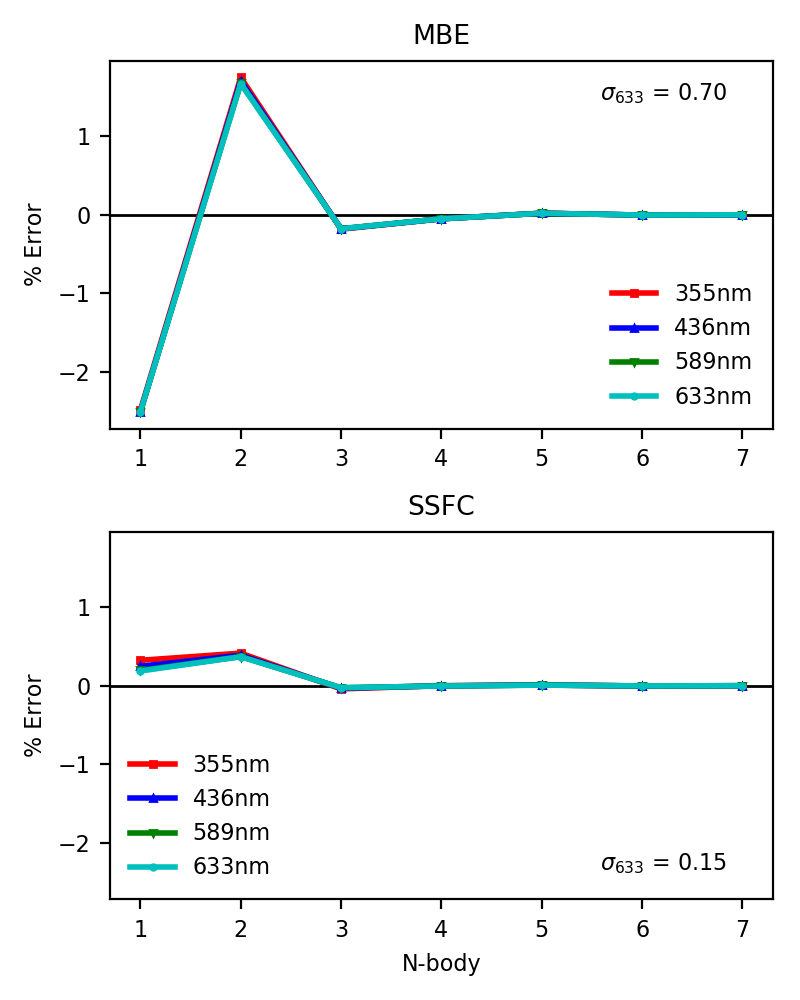
\includegraphics[scale=0.75]{p1/graphs/metthi_6_pol.png}
                \caption{(\textit{S})-methylthiirane}
                \label{metthi_6_pol}
            \end{subfigure}
            \begin{subfigure}{0.5\textwidth}
                \centering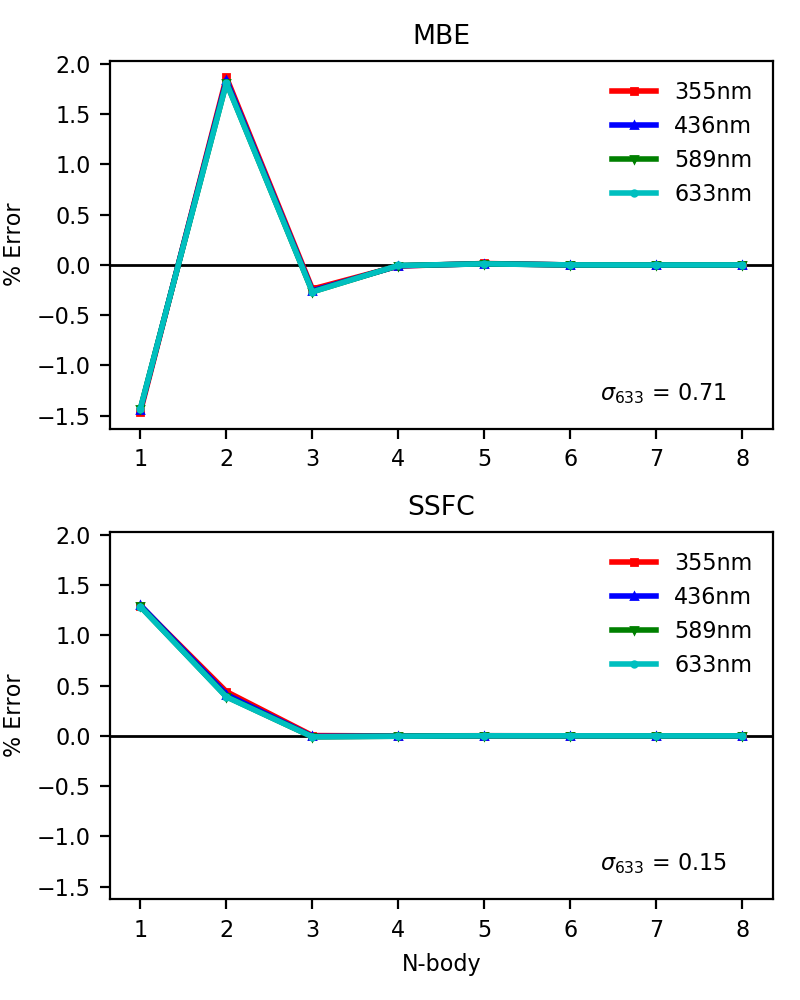
\includegraphics[scale=0.75]{p1/graphs/dma_7_pol.png}
                \caption{(\textit{M})-dimethylallene}
                \label{dma_7_pol}
            \end{subfigure}
            \caption{MBE and SSFC of dynamic polarizabilities for (a) (\textit{S})-methyloxirane in a seven-water solvent shell, (b) (\textit{S})-methylthiirane in a six-water solvent shell, and (c) (\textit{M})-dimethylallene in a seven-water solvent shell. Computed with CAM-B3LYP/aDZ.}
            \label{metox_metthi_dma_pol}
        \end{figure}
        For all three systems, the relatively large oscillations of the MBE for one- to four-body contributions were almost completely removed by SSFC, replacing the convergence trend with a nearly monotonic decaying function.  Analysis of a second snapshot taken from a molecular dynamics trajectory for (\textit{S})-methyloxirane and (\textit{S})-methylthiirane produce similar results (see the Supporting Information), with only that of (\textit{S})-methyloxirane exhibiting a slightly negative three-body term before reaching convergence.  In all three systems, the SSFC correction yields substantial improvement in the convergence of the MBE as compared to the uncorrected results, e.g.\ the standard deviation for (\textit{S})-methyloxirane decreases from 1.08 to only 0.22.

        Dynamic polarizabilities were also calculated for the larger 13-water (\textit{S})-methyloxirane system, as shown in Fig.\ \ref{metox_13_pol}. Oscillations to a higher error (up to 6\%) resulted in a higher standard deviation in this case than for the smaller solvent systems considered for the MBE.  However, the SSFC still dampened these oscillations significantly, with some small oscillations remaining. As with the electric dipole moment data considered earlier, BSSE is shown to be present and perhaps more important for properties than for interaction energies of the same system, with SSFC being a consistent method of reducing oscillations and speeding up convergence regardless of system size. 
        \begin{figure}
            \centering
            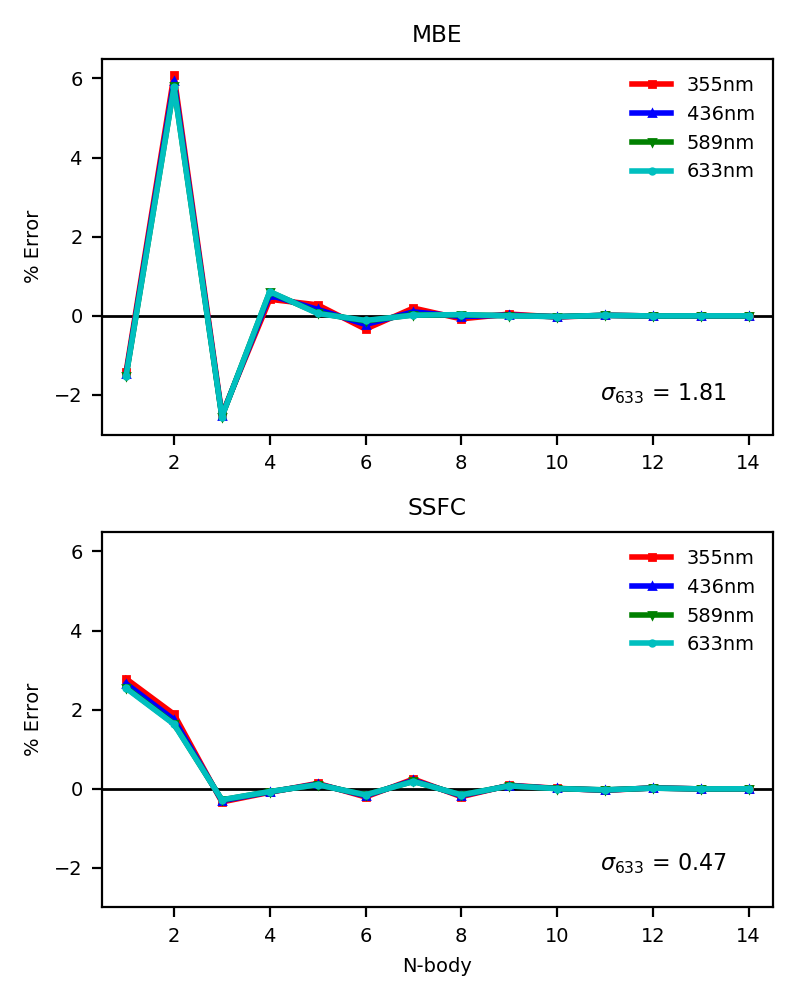
\includegraphics[scale=0.75]{p1/graphs/metox_13_pol.png}
            \caption{MBE and SSFC of dynamic polarizabilities for (\textit{S})-methyloxirane in a 13-water solvent shell. Computed with CAM-B3LYP/aDZ.}
            \label{metox_13_pol}
        \end{figure}

\subsection{Specific Rotations}

As stated previously, the properties considered thus far can be thought of as intrinsic to
the solute being perturbed by the solvent. MBEs for such properties, even beyond the energy,
still converge, and oscillations in the convergence for large clusters are mostly due to
BSSE and therefore can be corrected with CP-corrections such as SSFC or truncated schemes (such as VMFC(n)\cite{Kamiya2008} or MBCP(n)\cite{Richard2013}). It is shown that BSSE is perhaps more important in response property calculations; however, CP corrections still recover convergence within a three body approximation for even the largest solvent cluster considered. Next, the oscillatory convergence of the highly non-additive specific rotation of these clusters will be investigated, with the goal of deciding whether an MBE is an appropriate approximation even with a CP correction. 

The earlier work by Mach and Crawford\cite{Mach2014} identified specific rotations as a particular challenge for the MBE and its failure to converge with even small solvent shells suggested that BSSE was a potentially significant source of error. However, a number of other potential parameters exist that could also cause or exacerbate the observed erratic behavior for this property.  As Ouyang \textit{et al.} pointed out\cite{Ouyang2014}, oscillations in the MBE can occur due to successive sign-flips of terms with large errors; as a result, oscillations could potentially occur due to any large bias in the subsystem calculations. To that end, we selected (\textit{S})-methyloxirane and (\textit{S})-methylthiirane as representative cases for investigating various strategies for addressing these oscillations, though we also report results for (\textit{M})-dimethylallene at the B3LYP/aDZ and CAM-B3LYP/aDZ levels of theory.

One possible source of convergence problems for the MBE is noise due to the precision of the collected $\boldsymbol{G'}$ property tensor elements. Recent publications\cite{Richard2014,Liu2017a,Richard2018a} have taken notice of the effects of subsystem calculation convergence criteria and precision on higher-order terms in the MBE. Richard, Lao, and Herbert demonstrated in Ref.~\citenum{Richard2014} that precision errors in the energy rise rapidly for four- and five-body calculations as the total system size increases.  We accounted for this by using Gaussian's formatted checkpoint files for the data collection to ensure that we maintain full machine precision until the final result. Nevertheless, significant oscillations in the MBE results for specific rotations remained with little to no difference from the previous results\cite{Mach2014}, as shown in Fig.\ \ref{metox_metthi_rot}.  (\textit{NB} the significant difference in the vertical scale for the three test cases.)
        \begin{figure}
            \begin{subfigure}{0.5\textwidth}
                \centering 
                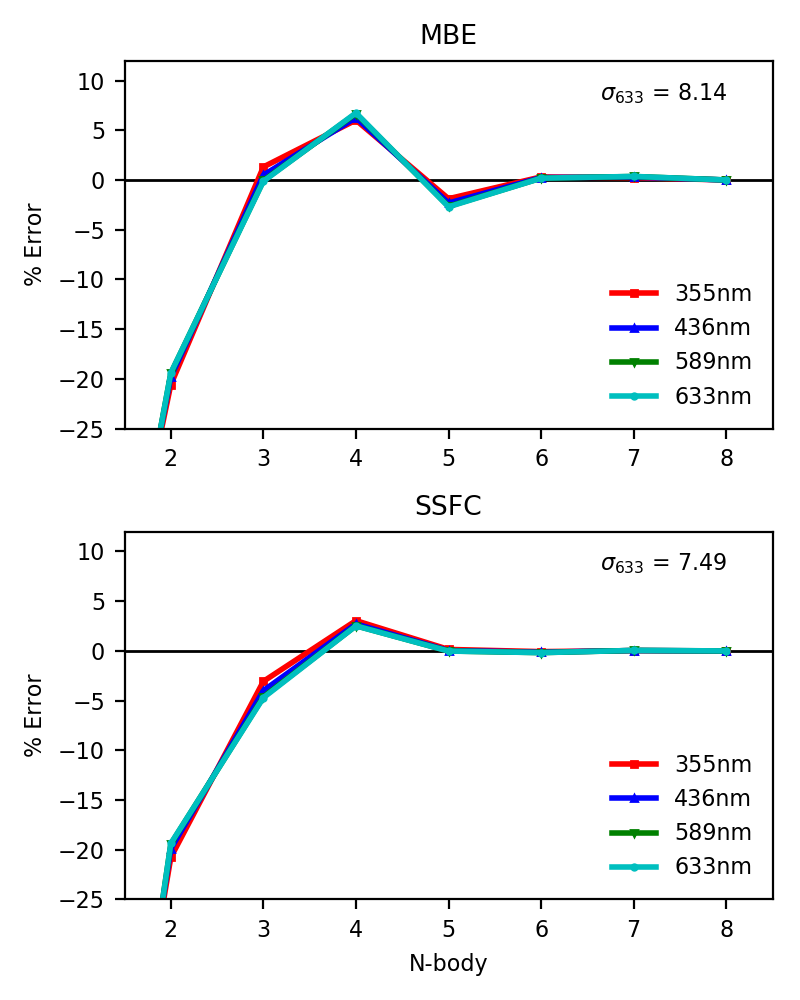
\includegraphics[scale=0.75]{p1/graphs/metox_7_b3_rot.png}
                \caption{(\textit{S})-methyloxirane}
                \label{metox_7_rot}
            \end{subfigure}%
            \begin{subfigure}{0.5\textwidth}
                \centering
                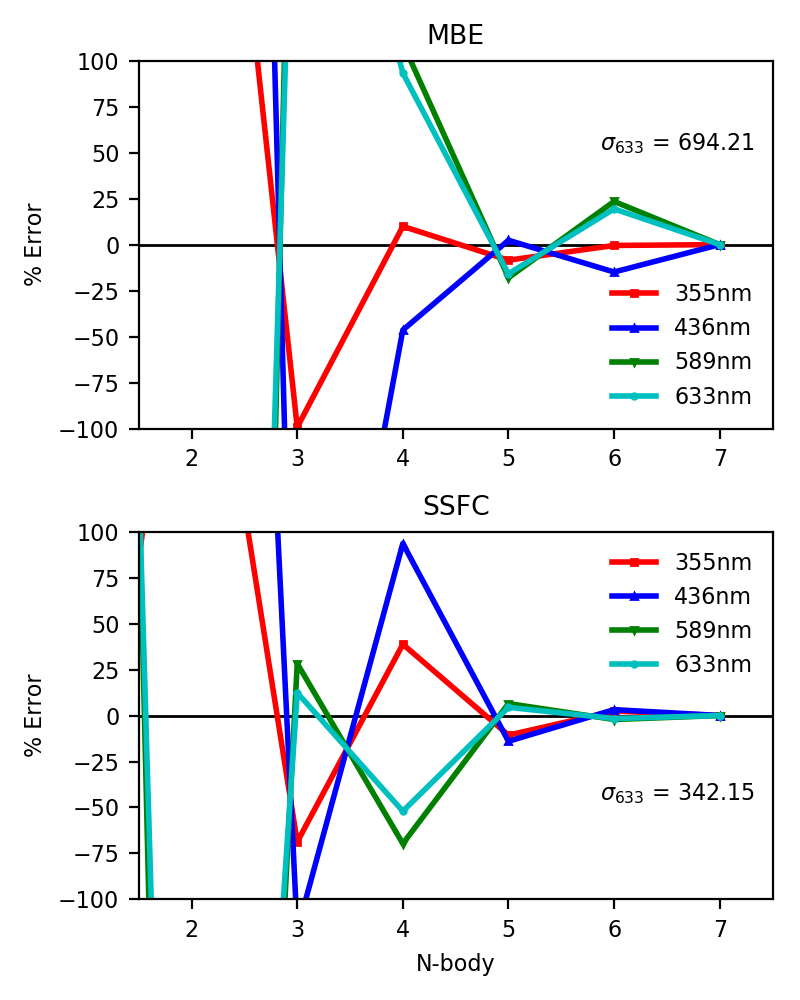
\includegraphics[scale=0.75]{p1/graphs/metthi_6_b3_rot.png}
                \caption{(\textit{S})-methylthiirane}
                \label{metthi_6_rot}
            \end{subfigure}
            \begin{subfigure}{0.5\textwidth}
                \centering
                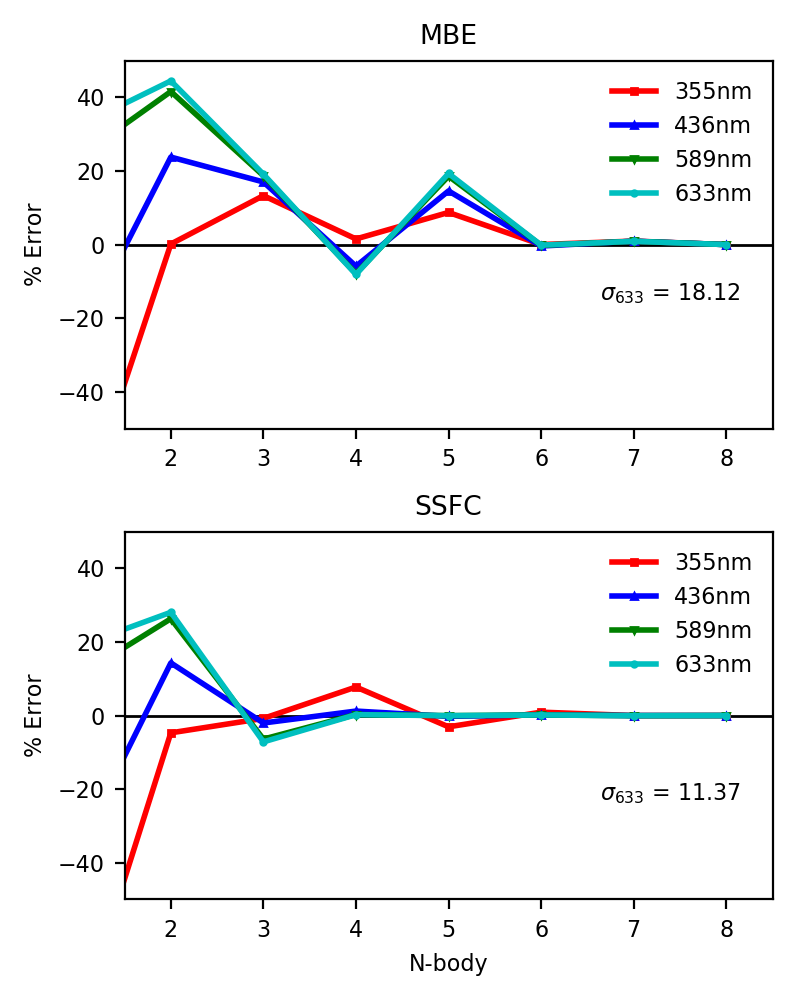
\includegraphics[scale=0.75]{p1/graphs/dma_7_b3_rot.png}
                \caption{(\textit{M})-dimethylallene}
                \label{dma_7_rot}
            \end{subfigure}
            \caption{MBE and SSFC of specific rotation for (a) (\textit{S})-methyloxirane in a seven-water solvent shell, (b) (\textit{S})-methylthiirane in a six-water solvent shell, and (c) (\textit{M})-dimethylallene in a seven-water solvent shell. Computed with B3LYP/aDZ.}
            \label{metox_metthi_rot}
        \end{figure}
        Indeed, the specific rotation of (\textit{S})-methylthiirane approaches 500\% error at the three-body contributions as compared to the converged results for the three longer wavelengths considered, in agreement with Table 8 of Ref.~\citenum{Mach2014}, and thus the precision of the individual terms is ruled out as a contributor to this behavior.

        A second potential source of MBE convergence error is the use of the relatively small aDZ basis set. Although this basis set has been found to be adequate for many applications in studies of optical activity, for some systems (notably, methylthiirane), larger basis sets are needed.\cite{Mach11,Howard2018a}  To investigate this issue, we carried out B3LYP/aTZ specific rotation calculations for both (\textit{S})-methyloxirane and (\textit{S})-methylthiirane, the results of which are presented in Fig.\ \ref{metox_metthi_rot_tz}.  For (\textit{S})-methyloxirane, the four- and five-body errors with the aDZ basis (Fig.\ \ref{metox_7_rot}) exhibit a significant oscillation from $\sim$7\% error to $\sim$-3\% error; the aTZ basis (Fig.\ \ref{metox_7_rot_tz}) reduces this somewhat to $\sim$5\% to -0.7\% error, and the two- to $n$-body standard deviation slightly decreases from 8.1 to 6.8\% error. Comparing Figs.\ \ref{metthi_6_rot} and \ref{metthi_6_rot_tz} for (\textit{S})-methylthiirane, increasing the basis set from aDZ to aTZ similarly offers no significant qualitative improvement, as errors vary wildly and are greater than 15\% for all wavelengths even at five-body contributions (and worse than the aDZ basis in some cases). The standard deviation at 633 nm does decrease from 694 to 159\% error with the improved basis set, though this is still well beyond acceptable limits and convergence with respect to $n$-body truncation remains strongly dependent on wavelength.
        \begin{figure}
            \begin{subfigure}{0.5\textwidth}
                \centering
                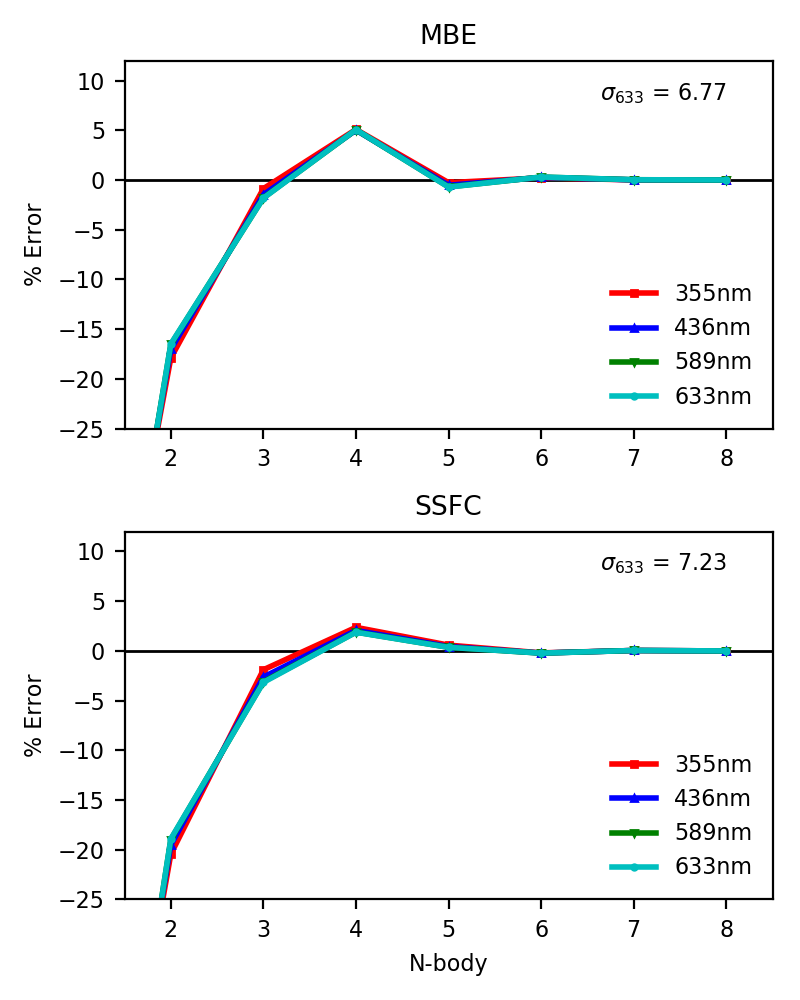
\includegraphics[scale=0.75]{p1/graphs/metox_7_tz_rot.png}
                \caption{(\textit{S})-methyloxirane}
                \label{metox_7_rot_tz}
            \end{subfigure}%
            \begin{subfigure}{0.5\textwidth}
                \centering
                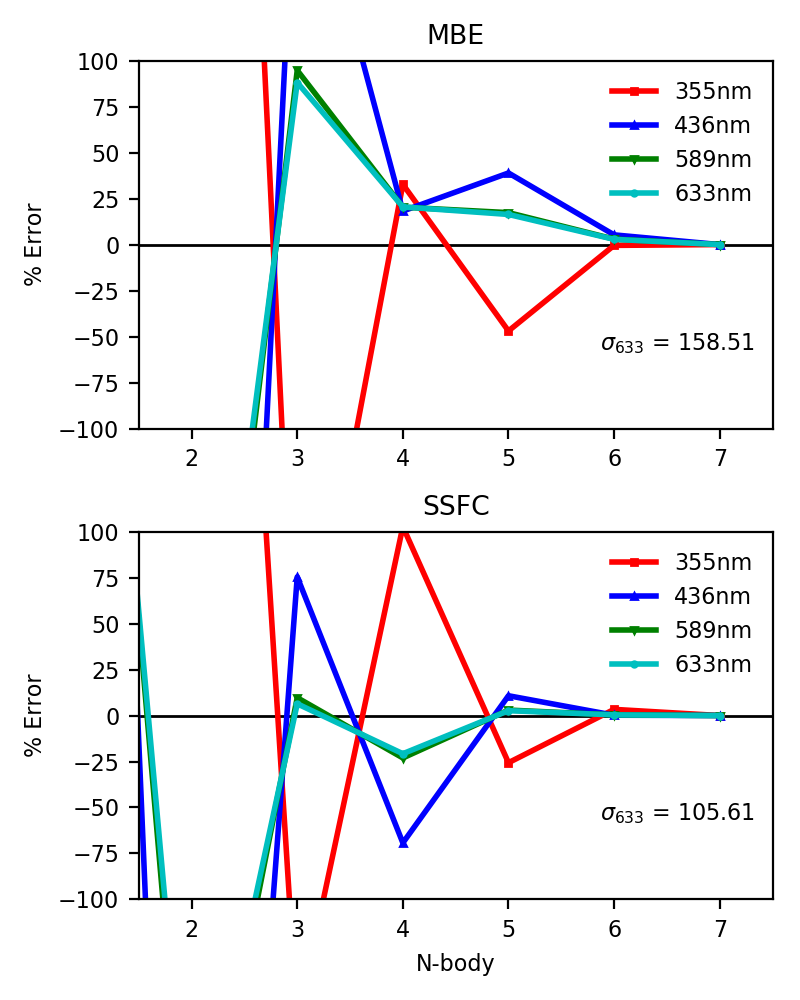
\includegraphics[scale=0.75]{p1/graphs/metthi_6_tz_rot.png}
                \caption{(\textit{S})-methylthiirane}
                \label{metthi_6_rot_tz}
            \end{subfigure}
            \caption{MBE and SSFC of specific rotation for (a) (\textit{S})-methyloxirane in a seven-water solvent shell and (b) (\textit{S})-methylthiirane in a six-water solvent shell. Computed with B3LYP/aTZ.}
            \label{metox_metthi_rot_tz}
        \end{figure}

        What about the choice of density functional?  While most studies to date have utilized the popular B3LYP functional, CAM-B3LYP has been proven useful to reduce errors in the near-resonance regions\cite{Peach2008,Lipparini2013} and to produce more consistent results with respect to wavelength, as shown in Fig.~\ref{dma_7_rot_cam}. While CAM-B3LYP for  (\textit{S})-methyloxirane does not yield significant differences in the MBE (cf.\ Fig.~\ref{metox_7_rot} with Fig.~7 of the Supporting Information), the change in functional makes a considerable difference for (\textit{S})-methylthiirane (Fig.~\ref{metthi_6_rot_cam}), as convergence trends were more consistent across all wavelengths tested. Nevertheless, the MBE still never converges to below 5\% error until the full expansion is reached, and a standard deviation of 461\% error was still observed (primarily due to the two-body error which is over 1000\% error). (\textit{M})-dimethylallene also exhibits more consistent convergence trends with CAM-B3LYP, with only a slightly increased standard deviation (18\% to 21\% error).

        \begin{figure}
            \begin{subfigure}{0.5\textwidth}
                \centering
                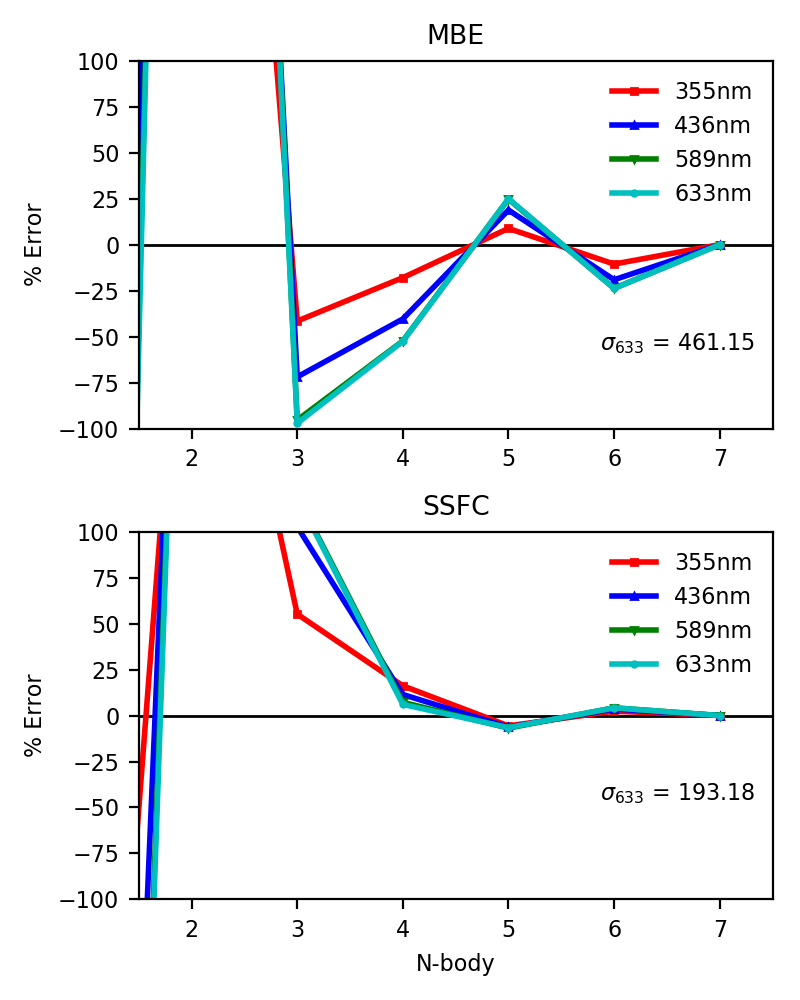
\includegraphics[scale=0.75]{p1/graphs/metthi_6_cam_rot.png}
                \caption{(\textit{S})-methylthiirane}
                \label{metthi_6_rot_cam}
            \end{subfigure}%
            \begin{subfigure}{0.5\textwidth}
                \centering
                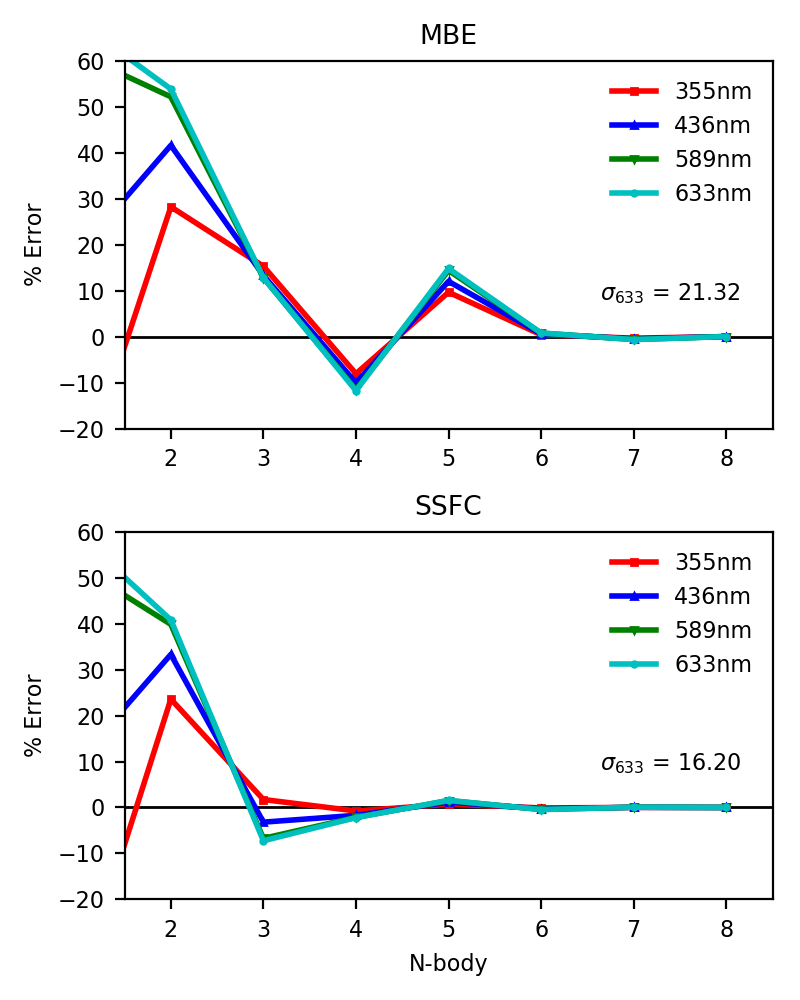
\includegraphics[scale=0.75]{p1/graphs/dma_7_cam_rot.png}
                \caption{(\textit{M})-dimethylallene}
                \label{dma_7_rot_cam}
            \end{subfigure}
            \caption{MBE and SSFC of specific rotation for (a) (\textit{S})-methylthiirane in a six-water solvent shell and (b) (\textit{M})-dimethylallene in a seven-water solvent shell. Computed with CAM-B3LYP/aDZ.}
            \label{metthi_dma_cam}
        \end{figure}

        The final non-BSSE issue considered is the choice of snapshot geometry. Calculations
of solvent-phase specific rotation based on MD trajectories typically employ a large number
of such snapshots, each with a distinct geometry that may be far from an energetic local
minimum.  Thus, we considered an additional snapshot for both (\textit{S})-methyloxirane and
(\textit{S})-methylthiirane in their seven- and six-water solvation shells respectively,
using CAM-B3LYP/aDZ (Fig.~\ref{snaps_2}). For (\textit{S})-methyloxirane, the MBE performs
somewhat worse for the new snapshot, with errors approaching from far below zero and
changing sign at the six-body level with errors of nearly 10\% still remaining, and a
considerably larger 22\% error standard deviation, though the same qualitative trends
appear. The new snapshot for (\textit{S})-methylthiirane, on the other hand, yields somewhat
better results, but again with the same qualitative trends.  The large errors near (and
over) 100\% seen previously are not present for this snapshot, though oscillations are still
clearly visible with respect to $n$-body truncation, as evidenced by the 4.9\% error
standard deviation. Additionally, the original 7-water (\textit{S})-methyloxirane snapshot
was edited to contain two short O...H bonds to test the effects of hydrogen bonding distance
on the convergence (compare Figs.~7 and 12 of the Supporting Information). As with the second snapshot, the same qualitative trends were observed, with very little difference in percent errors.

        \begin{figure}
            \begin{subfigure}{0.5\textwidth}
                \centering
                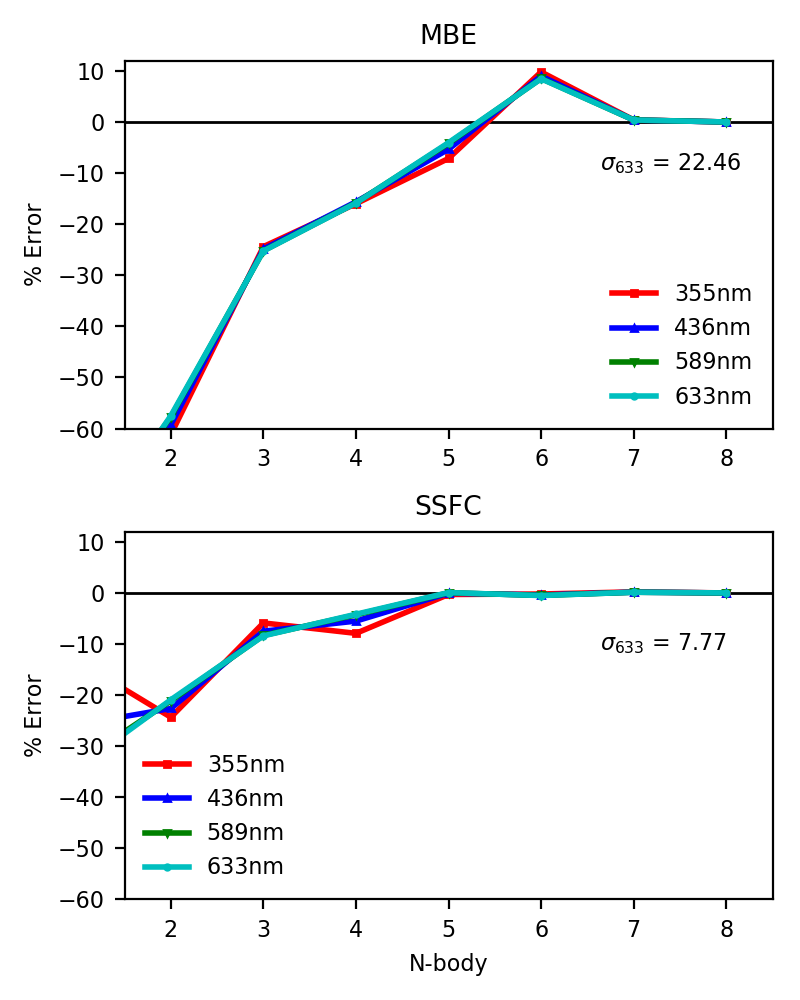
\includegraphics[scale=0.75]{p1/graphs/metox2_7_cam_rot.png}
                \caption{(\textit{S})-methyloxirane}
                \label{metox2_rot_cam}
            \end{subfigure}%
            \begin{subfigure}{0.5\textwidth}
                \centering
                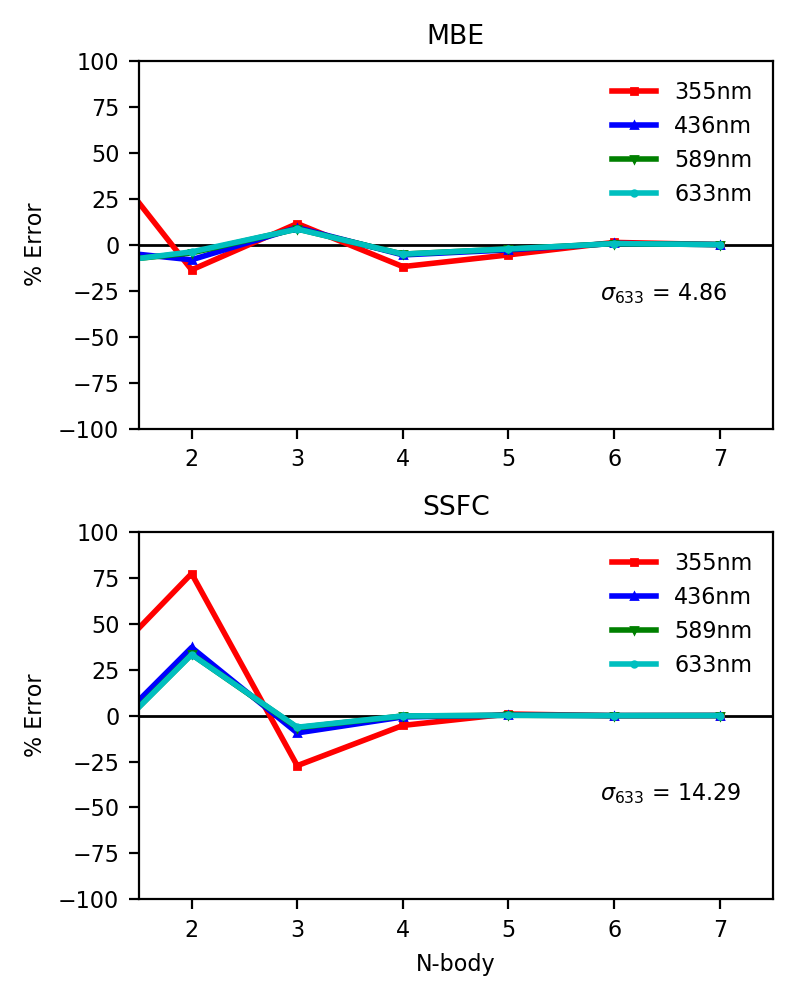
\includegraphics[scale=0.75]{p1/graphs/metthi2_6_cam_rot.png}
                \caption{(\textit{S})-methylthiirane}
                \label{metthi2_rot_cam}
            \end{subfigure}
            \caption{MBE and SSFC of specific rotation for additional snapshots of (a) (\textit{S})-methyloxirane in a seven-water solvent shell and (b) (\textit{S})-methylthiirane in a six-water solvent shell. Computed with CAM-B3LYP/aDZ.}
            \label{snaps_2}
        \end{figure}

        Next, in order to focus on the impact of BSSE on the MBE, we employed the SSFC CP-correction scheme in each of the test cases discussed above.  In all cases, the corrections reduce --- but do not eliminate --- the oscillations in the relative errors of the MBE, as evidenced by the lower frame of every sub-figure of Figs.~\ref{metox_metthi_rot}-\ref{snaps_2}.  Standard deviations also generally agree with this trend, with exceptions being Fig.~\ref{metox_7_rot_tz} and \ref{metthi2_rot_cam}.  In those two cases, the slightly higher two-body error in the SSFC case inflates the standard deviation, but from three-body onwards the oscillations are reduced.  For the smaller solvation shells of (\textit{S})-methyloxirane, (\textit{M})-dimethylallene, and (\textit{S})-methylthiirane, the convergence was also accelerated: by three- or four-body contributions, errors reasonable enough for predicting the sign of the optical rotation ($<$5\%) were achieved for most wavelengths with CAM-B3LYP/aDZ, though (\textit{S})-methylthiirane remains a challenge (16\% error at the four-body truncation for 355 nm), as well as 355 nm and 436 nm for the second methyloxirane snapshot (-8\% and -6\% at four-body). However, despite the relative improvements compared to the uncorrected MBE, these results do not imply that rapid convergence of even a CP-corrected MBE should be expected for highly non-additive properties such as specific rotation. Furthermore, a qualitative description of the specific rotation will not suffice: proper simulations of the property should be averaged over possibly hundreds of snapshots from an MD trajectory, and for complex systems with multiple chiral centers even a small error in the specific rotation can predict the wrong stereoisomer\cite{Fuentes18}. The fact that these trends also hold for (\textit{M})-dimethylallene speaks to the generality of the conclusions made thus far. Chirality in this compound is induced by a stereogenic axis, rather than a stereogenic center such as that in methyloxirane. In addition, the lowest energy excited states for dimethylallene are $\pi\rightarrow \pi^*$ valence transitions localized near the double bonds, as opposed to methyloxirane whose lowest excitation energies are Rydberg states\cite{Tam2004}. 
        
        The 13-water solvated (\textit{S})-methyloxirane in Fig.~\ref{metox_13_rot}, however, presents an even larger challenge, despite including the SSFC correction. Encouragingly, errors slightly above 5\% were found at the four-body truncation, but then the error continues to oscillate without converging until the 12-body truncation. While the SSFC greatly outperforms the uncorrected MBE in the five- to seven-body range (the MBE presents errors between 50 and 100\%, while SSFC presents $<$10\% in this range), it is actually worse from the nine-body truncation onwards. The eight-, nine-, and ten-body truncations increase substantially to roughly +/- 20\% error, while the MBE converged to $<$10\% by nine-body. This is one of the largest solvated property calculations performed with the MBE to date, and the results undermine its usefulness. This, combined with the substantial cost of the SSFC correction, greatly hinders the feasibility of the approach for production-level calculations of specific rotation for such large clusters, which may be necessary to properly model the effects of the solvent. 

        \begin{figure}
            \centering
            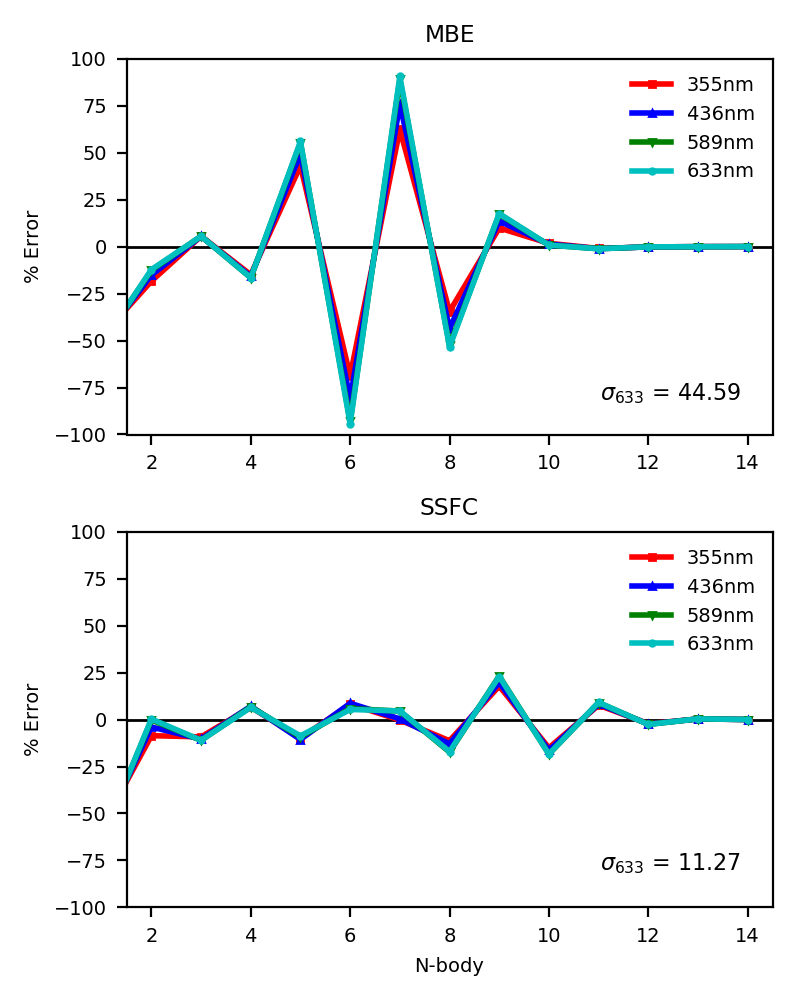
\includegraphics[scale=0.75]{p1/graphs/metox_13_rot.png}
            \caption{MBE and SSFC of specific rotation for (\textit{S})-methyloxirane in a 13-water solvent shell. Computed with CAM-B3LYP/aDZ.}
            \label{metox_13_rot}
        \end{figure}

        In cases of achiral solvents, such as water, one way to reduce the expense of the MBE for larger solvent shells is to include only contributions due to the solute and solute-solvent interactions. This is equivalent to restricting the sums in Eq.~(\ref{eq:mb_energy}) to only include fragments that contain the chiral solute. In principle, this should be advantageous for specific rotation calculations, as a pure achiral solvent (such as water) should give an optical rotation of zero upon averaging over a large number of snapshots and/or sufficiently large solvation clusters. Thus, neglecting solvent-solvent contributions should be of little consequence in the context of a sufficient MD trajectory while perhaps reducing the cost of the MBE through the removal of roughly half of the calculations needed for the full expansion of a solvated system (and much more for truncated expansions). For the smaller solvent shells of (\textit{S})-methyloxirane and (\textit{S})-methylthiirane (Fig.~\ref{slt}), the removal of solvent-solvent interactions has little impact from five-body interactions onwards.  However, the four-body approximation is slightly worsened even with the SSFC correction for (\textit{S})-methylthiirane (though the standard deviation decreases). Using this approach, the total number of calculations necessary for the full expansion decreases from 255 to 128 unique electronic structure calculations for (\textit{S})-methyloxirane, and, at any truncated $n$-body approximation, this number would decrease even more.  For large systems in which only a qualitative description of the specific rotation is necessary, these errors may be acceptable for such an improvement in the computational cost.

        \begin{figure}
            \begin{subfigure}{0.5\textwidth}
                \centering
                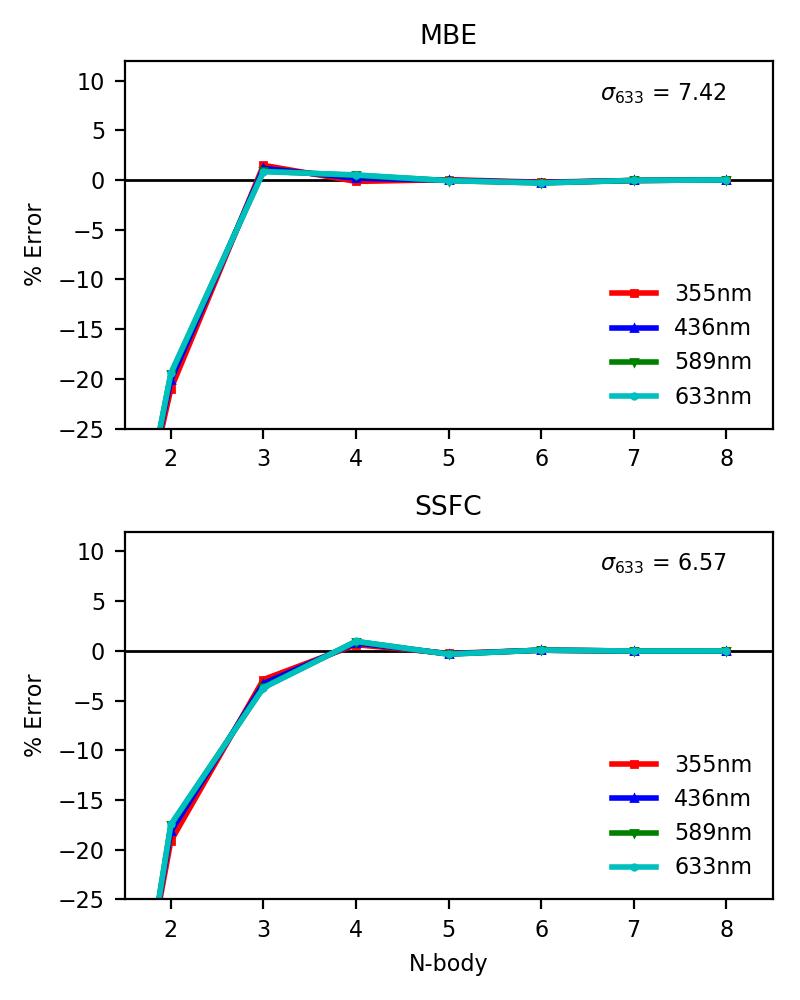
\includegraphics[scale=0.75]{p1/graphs/metox_7_slt_rot.png}
                \caption{(\textit{S})-methyloxirane}
                \label{metox_slt}
            \end{subfigure}%
            \begin{subfigure}{0.5\textwidth}
                \centering
                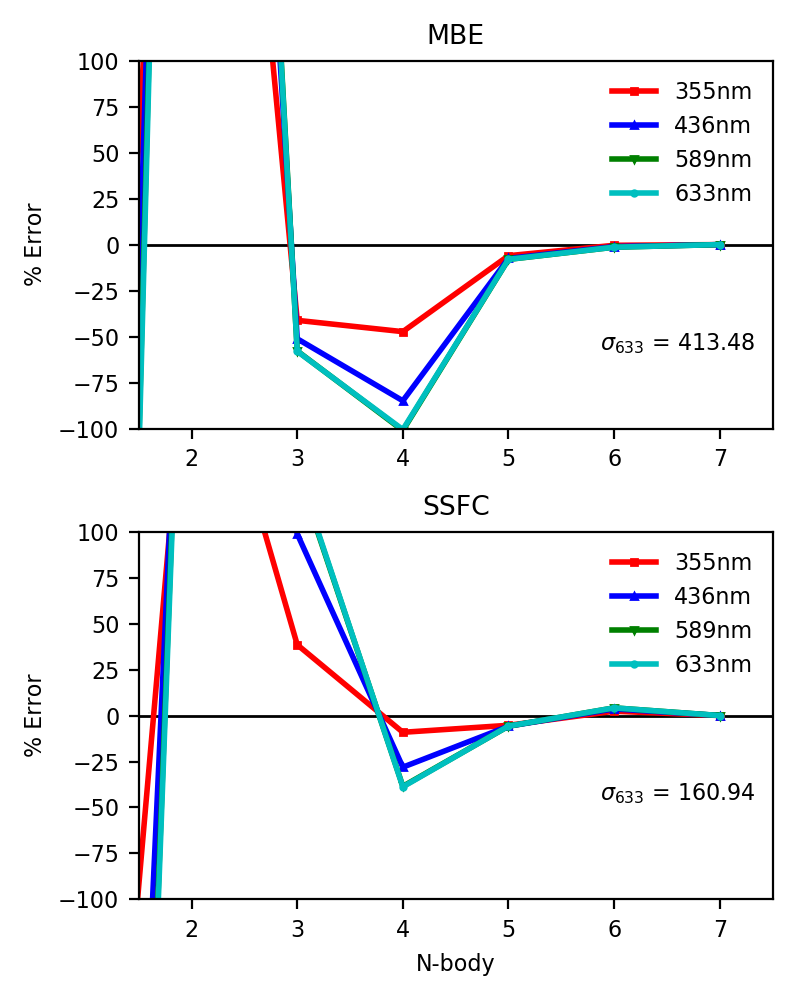
\includegraphics[scale=0.75]{p1/graphs/metthi_6_slt_rot.png}
                \caption{(\textit{S})-methylthiirane}
                \label{metthi_slt}
            \end{subfigure}
            \caption{MBE and SSFC of solute-fragment-only specific rotation for (a) (\textit{S})-methyloxirane in a seven-water solvent shell and (b) (\textit{S})-methylthiirane in a six-water solvent shell. Computed with CAM-B3LYP/aDZ.}
            \label{slt}
        \end{figure}

        In the case of the 13-water solvent shell for (\textit{S})-methyloxirane, excluding solvent-solvent interactions has a significant positive impact on the magnitude of oscillations in the MBE (Fig.~\ref{metox_13_slt}). While the standard deviation increases for the SSFC, the convergence in the troublesome eight- to ten-body range is improved, as compared to Fig.~\ref{metox_13_rot}.  Furthermore, the number of unique electronic structure calculations for the full expansion reduces by roughly a factor of two --- 16383 to 8192 --- with massive savings possible for truncated expansions. Still, due to the significant non-BSSE oscillations in the MBE, the possibility of false convergence, and the prohibitive cost of the SSFC correction, a CP-corrected MBE cannot be recommended as a reliable low-cost quantitative approximation to the specific rotation of the full-cluster. 

        \begin{figure}
            \centering
            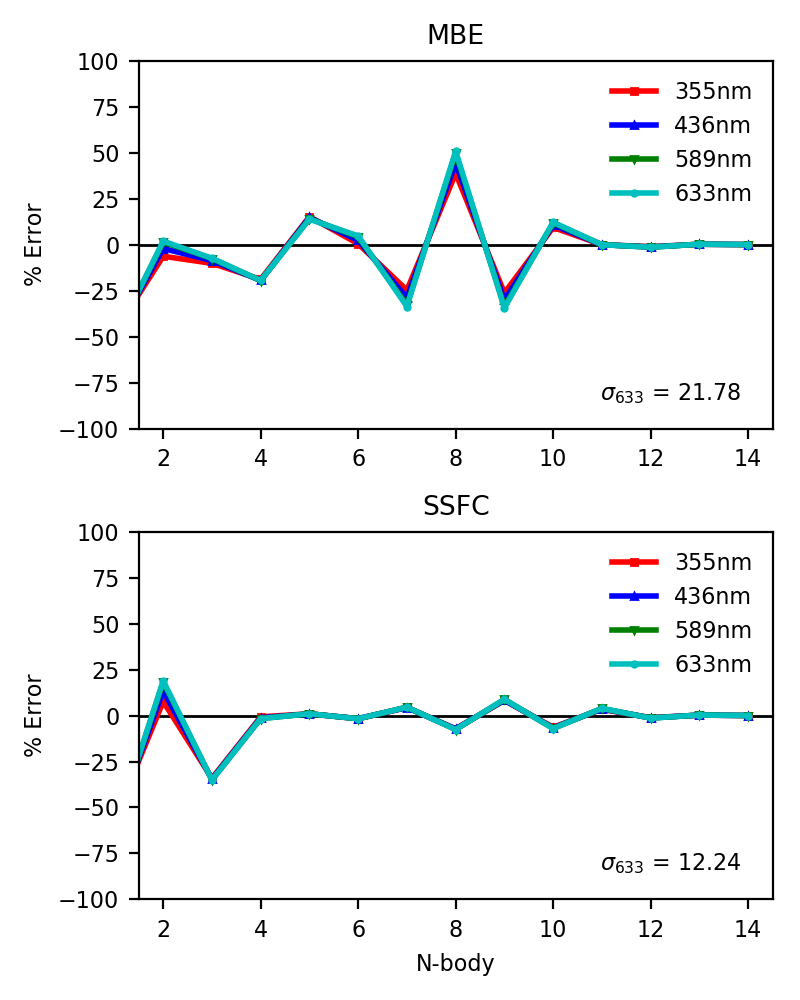
\includegraphics[scale=0.75]{p1/graphs/metox_13_slt_rot.png}
            \caption{MBE and SSFC of solute-fragment-only specific rotation for (\textit{S})-methyloxirane in a 13-water solvent shell. Computed with CAM-B3LYP/aDZ.}
            \label{metox_13_slt}
        \end{figure}
